\documentclass[tikz,border=5mm]{standalone}
\usepackage{tikz}
\usetikzlibrary{positioning,arrows.meta}
\usepackage{xcolor}

% Define colors
\definecolor{nodefcolor}{RGB}{220,53,69}
\definecolor{patterncolor}{RGB}{255,193,7}
\definecolor{policycolor}{RGB}{0,123,255}
\definecolor{provsafecolor}{RGB}{40,167,69}
\definecolor{gridcolor}{RGB}{200,200,200}

\begin{document}
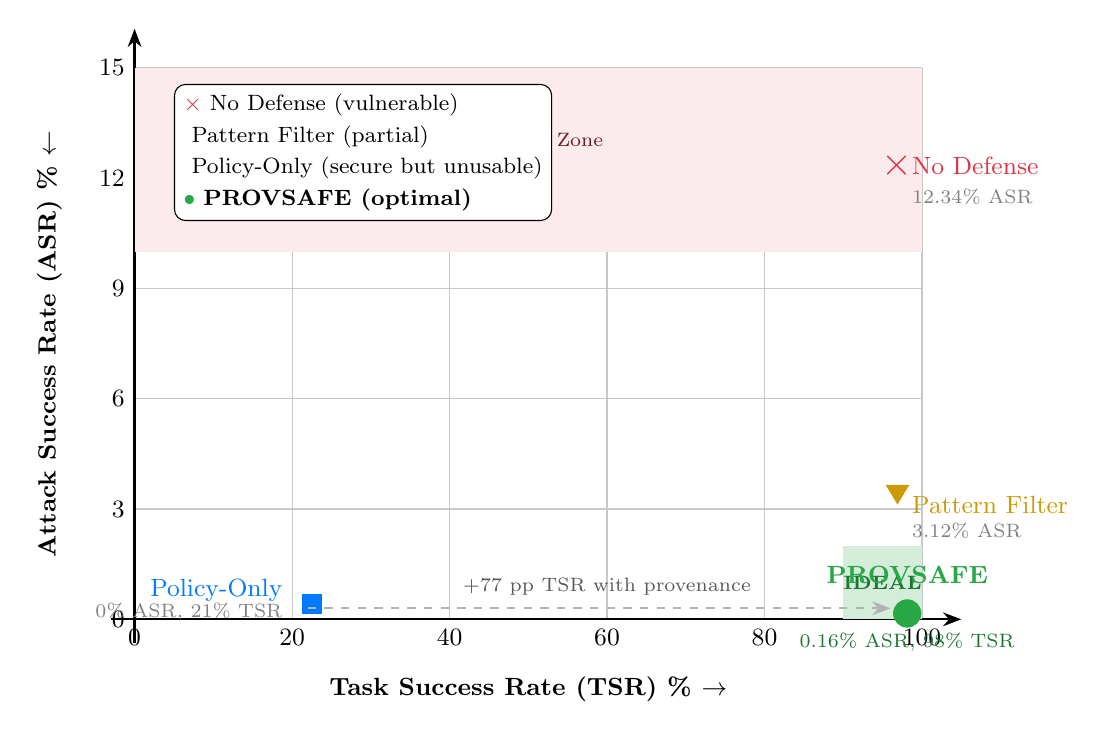
\begin{tikzpicture}[
    >=Stealth
]

% Grid dimensions: 10cm x 7cm
% X axis: TSR 0-100%, scaled to 10cm
% Y axis: ASR 0-15%, scaled to 7cm (0.467cm per %)

\def\xscale{0.1}  % 10cm / 100%
\def\yscale{0.467} % 7cm / 15%

% Draw grid
\foreach \x in {0,20,40,60,80,100} {
    \draw[gridcolor] (\x*\xscale, 0) -- (\x*\xscale, 15*\yscale);
    \node[below, font=\small] at (\x*\xscale, 0) {\x};
}
\foreach \y in {0,3,6,9,12,15} {
    \draw[gridcolor] (0, \y*\yscale) -- (100*\xscale, \y*\yscale);
    \node[left, font=\small] at (0, \y*\yscale) {\y};
}

% Axes
\draw[->, thick] (-0.3,0) -- (10.5,0);
\draw[->, thick] (0,-0.3) -- (0,7.5);

% Axis labels
\node[below, font=\small\bfseries] at (5, -0.6) {Task Success Rate (TSR) \% $\rightarrow$};
\node[left, font=\small\bfseries, rotate=90, anchor=south] at (-0.8, 3.5) {Attack Success Rate (ASR) \% $\leftarrow$};

% Ideal region
\fill[provsafecolor!20] (90*\xscale, 0) rectangle (100*\xscale, 2*\yscale);
\node[font=\scriptsize\bfseries, provsafecolor!70!black] at (95*\xscale, 1*\yscale) {IDEAL};

% Dangerous region
\fill[nodefcolor!10] (0, 10*\yscale) rectangle (100*\xscale, 15*\yscale);
\node[font=\scriptsize, nodefcolor!50!black] at (50*\xscale, 13*\yscale) {High Risk Zone};

% Data points
% No Defense: TSR=96.88, ASR=12.34
\node[nodefcolor, font=\Large] at (96.88*\xscale, 12.34*\yscale) {$\times$};
\node[anchor=west, font=\small, nodefcolor] at (97.5*\xscale, 12.34*\yscale) {No Defense};
\node[anchor=west, font=\scriptsize, gray] at (97.5*\xscale, 11.5*\yscale) {12.34\% ASR};

% Pattern Filter: TSR=96.88, ASR=3.12
\fill[patterncolor!80!black] (96.88*\xscale, 3.12*\yscale) -- ++(0.15,0.25) -- ++(-0.3,0) -- cycle;
\node[anchor=west, font=\small, patterncolor!80!black] at (97.5*\xscale, 3.12*\yscale) {Pattern Filter};
\node[anchor=west, font=\scriptsize, gray] at (97.5*\xscale, 2.4*\yscale) {3.12\% ASR};

% Policy-Only: TSR=21.25, ASR=0.00
\fill[policycolor] (21.25*\xscale, 0.15*\yscale) rectangle ++(0.25, 0.25);
\node[anchor=east, font=\small, policycolor] at (20*\xscale, 0.8*\yscale) {Policy-Only};
\node[anchor=east, font=\scriptsize, gray] at (20*\xscale, 0.2*\yscale) {0\% ASR, 21\% TSR};

% PROVSAFE: TSR=98.12, ASR=0.16
\fill[provsafecolor] (98.12*\xscale, 0.16*\yscale) circle (0.18);
\node[anchor=south, font=\small\bfseries, provsafecolor] at (98.12*\xscale, 0.7*\yscale) {PROVSAFE};
\node[anchor=north, font=\scriptsize, provsafecolor!70!black] at (98.12*\xscale, -0.1*\yscale) {0.16\% ASR, 98\% TSR};

% Arrow showing improvement
\draw[->, thick, gray!60, dashed] (22*\xscale, 0.3*\yscale) -- (96*\xscale, 0.3*\yscale);
\node[above, font=\scriptsize, gray!70!black] at (60*\xscale, 0.4*\yscale) {+77 pp TSR with provenance};

% Legend box
\node[draw, rounded corners, fill=white, font=\footnotesize, align=left, anchor=north west] at (0.5, 6.8) {
    \textcolor{nodefcolor}{\textbf{$\times$}} No Defense (vulnerable)\\[2pt]
    \textcolor{patterncolor!80!black}{$\blacktriangle$} Pattern Filter (partial)\\[2pt]
    \textcolor{policycolor}{$\blacksquare$} Policy-Only (secure but unusable)\\[2pt]
    \textcolor{provsafecolor}{$\bullet$} \textbf{PROVSAFE (optimal)}
};

\end{tikzpicture}
\end{document}
